\documentclass[a4paper,11pt]{article}
%Packet section
\usepackage[utf8]{inputenc}
\usepackage[style=ieee]{biblatex}
\usepackage{csquotes}
\usepackage[top=2.5cm,bottom=2.5cm,left=2cm,right=2cm]{geometry}
\usepackage[english]{babel}
\usepackage{float}
\usepackage{caption}
\usepackage{pdfpages} % Para insertar la portada en formato PDF.
\usepackage[hidelinks]{hyperref} % Para urls.
\usepackage{longtable} % Para tablas largas.
\usepackage{graphicx} % Para cargar imagenes
\usepackage{titlesec}
\usepackage{fancyhdr}
\usepackage[parfill]{parskip}
\usepackage[acronym,nogroupskip]{glossaries}
\usepackage{todonotes}
\usepackage{dirtree}
\usepackage{subcaption}
\usepackage{mathtools}
\usepackage{amsmath}
\usepackage{multirow}
\usepackage{algpseudocodex}
\usepackage{algorithm}
\usepackage{listings}
\usepackage{bytefield}
\raggedbottom

\addbibresource{SensorNetworks.bib}

%Eliminar la sangría y otros ajustes de los headers
\setlength{\parindent}{0px}
\setlength{\headheight}{13.07225pt}
%Glosaries
\makenoidxglossaries

\newacronym{iot}{IoT}{Internet of Things}
\newacronym{mcu}{MCU}{MicroController Unit}
\newacronym{lorawan}{LoRaWAN}{Long Range Wide Area Network}
\newacronym{spi}{SPI}{Serial Peripheral Interface}
\newacronym{fsk}{FSK}{Frecuency Shift Keying}
\newacronym{gfsk}{GFSK}{Gaussian Frecuency Shift Keying}
\newacronym{msk}{MSK}{Minimum-Shift Keying}
\newacronym{gmsk}{GMSK}{Gaussian Minimum-Shift Keying}
\newacronym{rf}{RF}{Radio Frecuency}
\newacronym{gnss}{GNSS}{Global Navigation Satellite System}
\newacronym{ble}{BLE}{Bluetooth Low Energy}
\renewcommand*\glspostdescription{\hfill}
\newcommand\acrfullr[2][]{\acrshort[#1]{#2} (\acrlong[#1]{#2})}


%New page styles
\fancypagestyle{specialpage}{
  \fancyhf{}
  \fancyhead[L]{}
  \fancyhead[R]{\textit{GLOSARY}}
  \fancyfoot[L]{}
  \fancyfoot[OR]{\thepage}
}
\fancypagestyle{indicefig}{
  \fancyhf{}
  \fancyhead[L]{}
  \fancyhead[R]{\textit{LIST OF FIGURES AND TABLES}}
  \fancyfoot[L]{}
  \fancyfoot[R]{\thepage}
}
\fancypagestyle{abstract}{
    \fancyhf{}
    \renewcommand{\headrulewidth}{0pt} % Asegurarse de que la barra negra también se elimine en esta página
    \fancyfoot[EL]{\thepage}
    \fancyfoot[OR]{\thepage}
}

%Tools to write code directly into the document.
\lstset{
    language=C++,         
    basicstyle=\ttfamily,
    numbers=left,
    numberstyle=\tiny,
    stepnumber=1,
    frame=single,
    tabsize=4,
    breaklines=true,
    captionpos=b,
    showspaces=false,
    showstringspaces=false
}


\title{Sensor Networks: Project 1}
\author{Diego Aceituno Seoane}
\date{December 2024}

\begin{document}
\begin{titlepage}
    \raggedleft
    \rule{2pt}{\textheight}
    \hspace{0.05\textwidth}
    \parbox[b]{0.9\textwidth}{
            {\Huge\bfseries LoRaWAN communications for a plant monitoring IoT System}\\[\baselineskip] % Title
            {\Large\textit{Project documentation}}\\[7\baselineskip] % Subtitle or further description
        \vspace{0.45\textheight}
        
        {\Large\textsc{Diego\ Aceituno\ Seoane}}\\[1.5\baselineskip]
        \vspace{0.05\textheight}
        
        {\noindent\large Sensor Networks}\\
        {\noindent\large Fall 2024}\\
    }
\end{titlepage}
\clearpage
\pagestyle{fancy}
\fancyfoot{}
\fancyhead[L]{}
\fancyfoot[L]{}
\fancyfoot[R]{\thepage}
\setcounter{tocdepth}{2}
\tableofcontents
\clearpage
\thispagestyle{indicefig}
\listoffigures
\listoftables
\clearpage
\section*{GLOSARY} % Glosario
\thispagestyle{specialpage}
\printnoidxglossary[style=list,type=\acronymtype,title=] % Acrónimos
\clearpage
\fancyhead[R]{\textit{INTRODUCTION}}
\section{INTRODUCTION}

This document presents the report of the first project developed for the "Sensor Networks" course.

The project is based around the study of wireless sensors design and the implementation of a use case in order to obtain data from remote sensors, applying knowledge in communication protocols and in low capabilities platforms.

The system is centered around a solution designed in a previous course (Embedded platforms and communications for \acrfullr{iot}). In the course, a solution to obtain biological data from a plant and other parameters such as the 
GPS location was designed. This solution is presented in the \autoref{fig:solutionIntro} and uses the \texttt{DISCO-L072CZ-LRWAN1} board.
\begin{figure}[H]
    \centering
    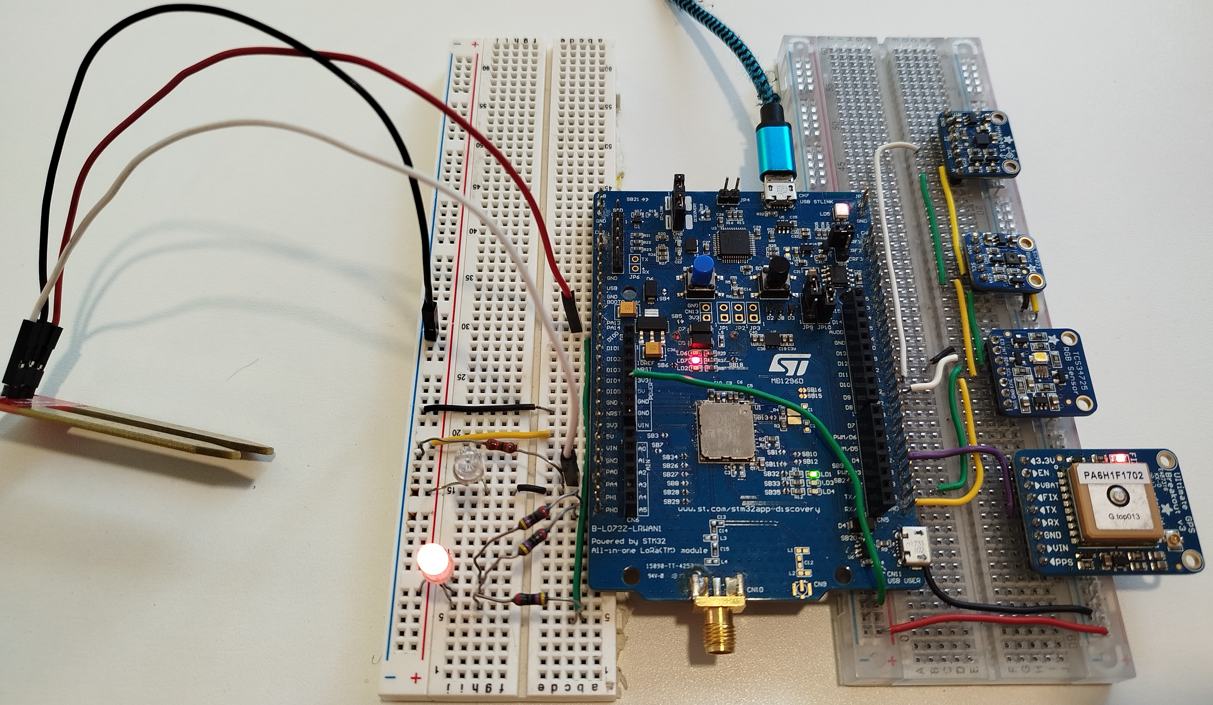
\includegraphics[width=0.53\textwidth]{images/1/sistema.png}
    \caption{Solution developed in the previous course.}
    \label{fig:solutionIntro}
\end{figure}

To further expand on this idea, the task presented is to modify the system and send the data with wireless communications to allow the final user to see all the information needed regarding the status of the plant 
remotely. To achieve this, the \acrfullr{lorawan} module of the board is used. This module combined with a event queue based solution will send the information of the plant to 
a remote gateway and routed to a network server that will process the data into a dashboard.

The final dashboard that presents the information obtained is is presented in \autoref{fig:finalDashboard}.
\begin{figure}[H]
    \centering
    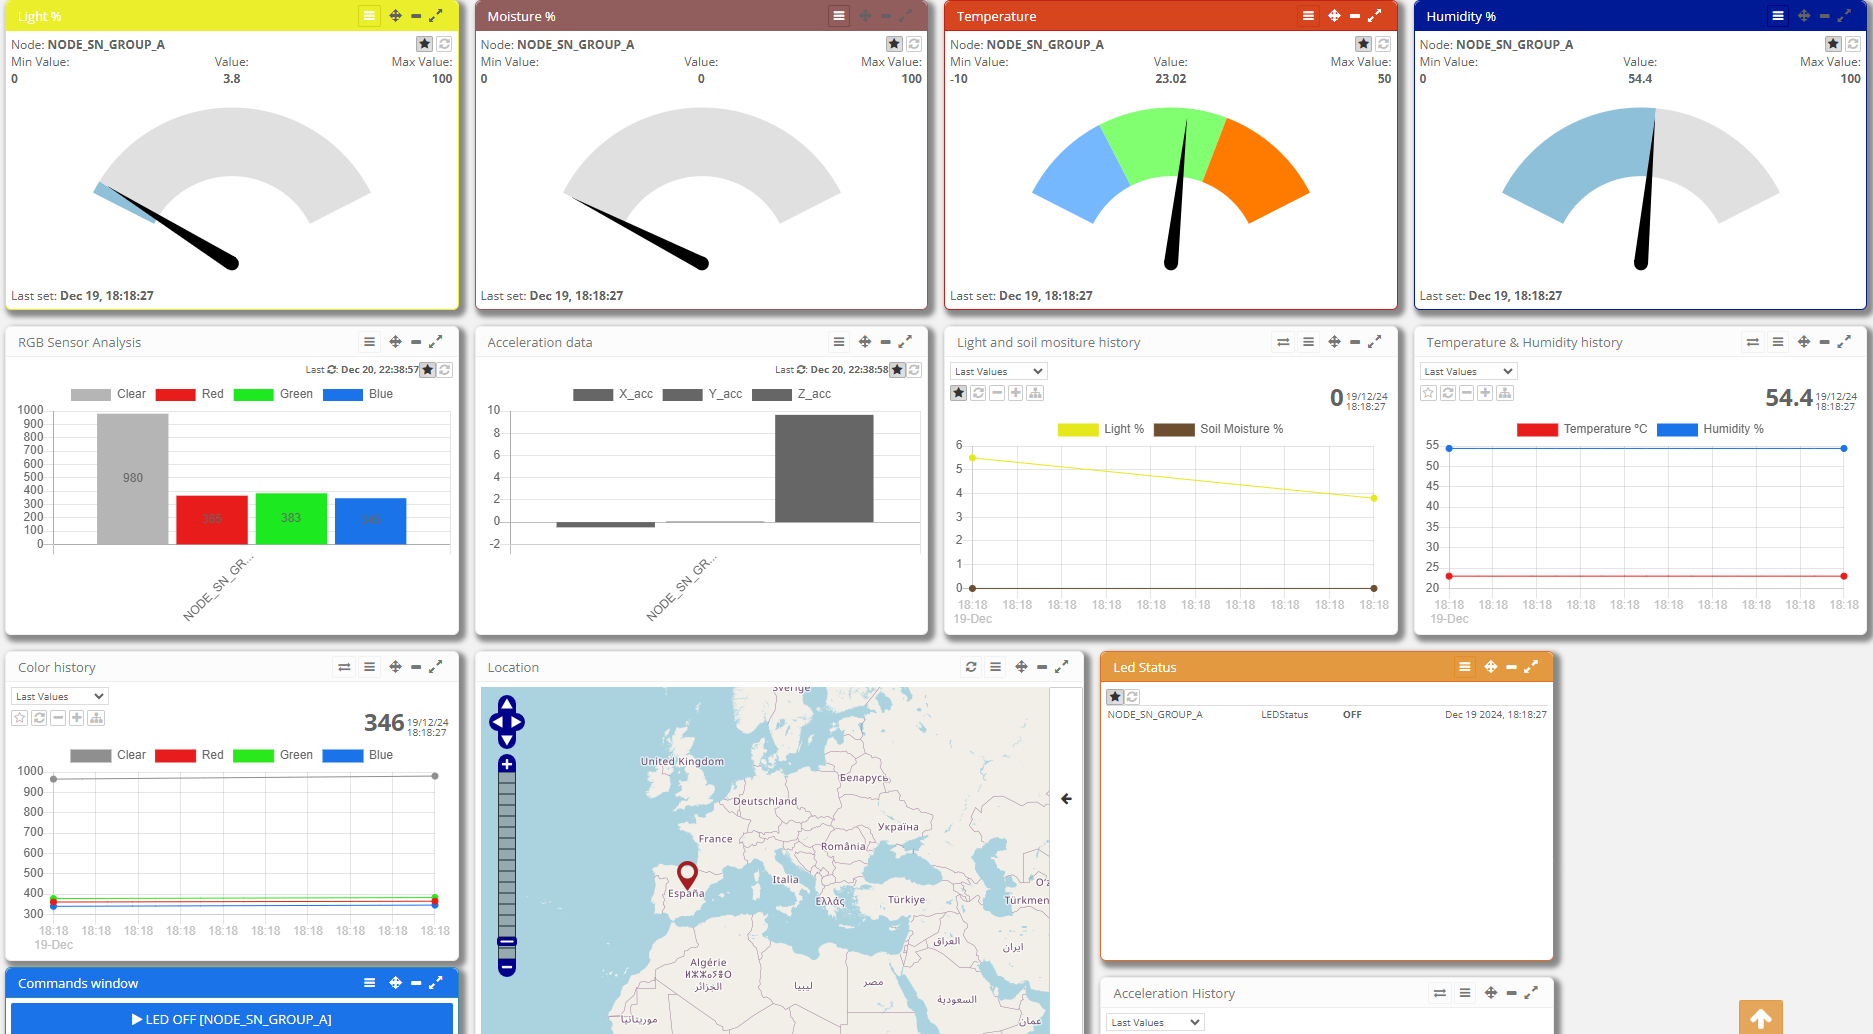
\includegraphics[width=0.8\textwidth]{images/1/FinalDashboard.png}
    \caption{Final dashboard of the system.}
    \label{fig:finalDashboard}
\end{figure}
\clearpage
\fancyhead[R]{\textit{REQUIREMENTS ANALYSIS}}
\section{REQUIREMENTS ANALYSIS}
\subsection{Specifications required and implemented}

This section presents in the next tables the list of requirements needed to implement, as well as the implementation status for each specification.
\vspace{2\baselineskip}
\begin{table}[H]
    \begin{center}
        \begin{tabular}{|p{0.1\textwidth} | p{0.7\textwidth} | p{0.15\textwidth}|}
            \hline
            \textbf{Req. ID} & \textbf{Requirement description} & \textbf{Implemented}\\
            \hline
            Phase2.1 & The target must be able to send the location. & Yes\\
            \hline
            Phase2.2 & The target must be able to send, apart from the location, 3 environmental parameters. & Yes\\
            \hline
            Phase2.3 & The dashboard must have a widget to represent the previous parameters values. & Yes\\
            \hline
            Phase2.4 & The dashboard must allow the user to send commands to change the RGB Led. The commands should be: ``OFF'', ``Green'' and ``Red''.  & Yes\\
            \hline
        \end{tabular} 
    \end{center}
    \caption{Phase 2 requirements implementation status}
    \label{ReqGeneral}
\end{table}

\vspace{2\baselineskip}

\begin{table}[H]
    \begin{center}
        \begin{tabular}{|p{0.1\textwidth} | p{0.7\textwidth} | p{0.15\textwidth}|}
            \hline
            \textbf{Req. ID} & \textbf{Requirement description} & \textbf{Implemented}\\
            \hline
            Phase3.1 & Get all the parameters from the sensors. & Yes\\
            \hline
            Phase3.2 & Convert the data format of the system parameters from string to the most appropriate type to reduce their length. & Yes\\
            \hline
            Phase3.3 & Modify the LUA code to retrieve the values of all the parameters. & Yes\\
            \hline
        \end{tabular} 
    \end{center}
    \caption{Optional requirements implementation status}
    \label{ReqTest}
\end{table}

\subsection{Extra specifications implemented}

To further expand the communication capabilities of the system, a frame header was implemented. This allows for:
\begin{itemize}
    \item Frame version.
    \item Control and data separation.
    \item Scalability.
\end{itemize}

The design for this is described in a specific \hyperref[header]{chapter} of the document.
\clearpage
\fancyhead[R]{\textit{NODE SOFTWARE}}
\section{NODE SOFTWARE}

\subsection{Description of the implementation}

The system extends the functionality of the Mbed-OS \acrshort{lorawan} example provided by the teachers, in which an event-queue is provided.

ThIS event-queue provides an asynchronous event dispatcher, in this case for \acrshort{lorawan} events. And, for any event that happens in the system, a callback will be done to process that situation. This working can be seen in the next figure.

\begin{figure}[H]
    \centering
    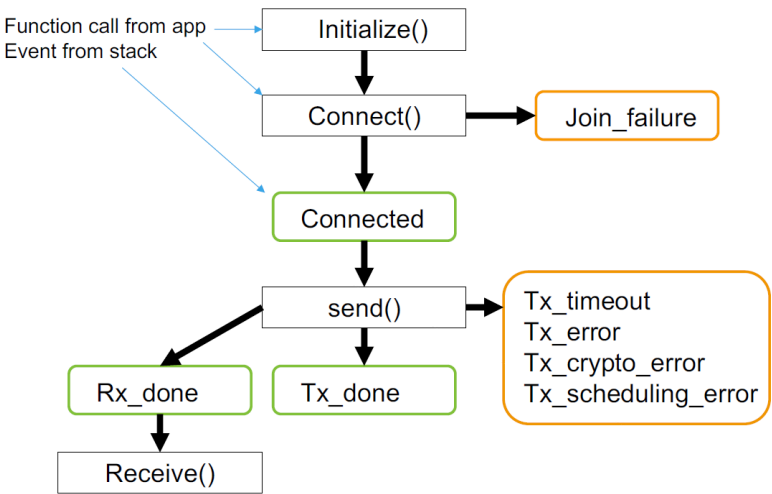
\includegraphics[width=0.6\textwidth]{images/4/event-queue.png}
    \caption{EventQueue process\cite{SensorNetworksProject1_slides_2024}}
    \label{fig:events}
\end{figure}

The solution is implemented by extending the previous event-queue. This event queue will detect possible TX windows in the \acrshort{lorawan} PHY layer and create an event to send a new message with data regarding the measurements of the plant sensors. These sensors are: 
GPS, brightness, soil moisture, humidity, temperature, linear acceleration, RGB data and led status.

To obtain this data, measurement threads are changed from the previous project, these threads read new values each 5 seconds and store the data in an mutex-controlled structure. This structure is later used when the \acrshort{lorawan} stack detects a possible transmitting window.

The threads defined for the solution are:
\begin{itemize}
    \item Main thread with the event-queue.
    \item I2C thread.
    \item GPS thread.
\end{itemize}
\subsection{Modules}
The modules used for this project are mainly the same from the previous course project, with the only exception being a new module to allocate the shared data for the communication between threads.

The module are also used by the same threads:
\begin{itemize}
    \item The I2C thread communicates with the accelerometer, temperature \& humidity and the color module.
    \item The GPS thread controls only the GPS module.
\end{itemize}

\clearpage
\subsection{Threads and communication design} % Comentar los cambios realizados

\acrshort{lorawan} is used, which analyzes a possible transmitting window for the next message. Because of this, a method is needed that ensures the maximum utilization of these windows without depending on the main thread. The final design for this can be seen in the next figure.

\begin{figure}[H]
    \centering
    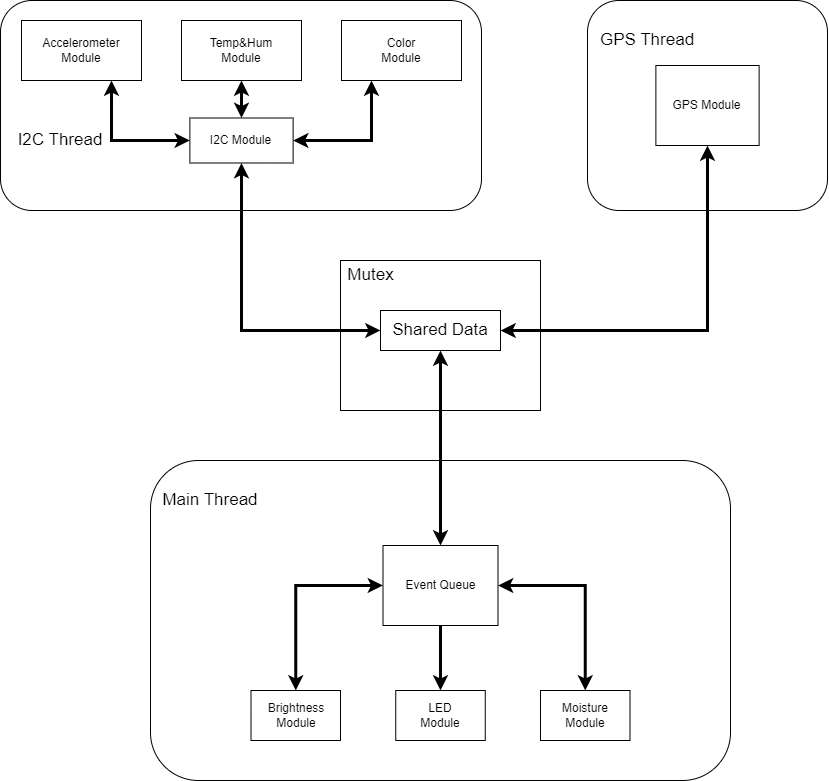
\includegraphics[width=0.85\textwidth]{images/4/Modules.png}
    \caption{Final module design for the system}
    \label{fig:modules}
\end{figure}
In the previous project, the approach was having the main thread controlling the execution of the measuring threads with signals. In this project, that won't work because the main thread is controlled by the event-queue. 
To solve this and taking into account the best-effort nature of the system, the decision was to make the measuring threads run independently of the main thread, waking themself up every \texttt{N} seconds. 

The communication between the measuring threads and the main thread had to be redone as well, as in the previous project used an intermediate queue. In this system that could create problems in the next events:
\begin{itemize}
    \item The system doesn't control the time between readings of the data, so there's a possibility of filling of the queue.
    \item The system only focuses on sending the last measurements possible for each sensor, so there's no need for previous data that isn't processed.
\end{itemize}

To solve all this situation, the communication was reduced to a shared structure that contains all the necessary data that is going to be sent through \acrshort{lorawan}. The access to this common structure is done using a Mbed-OS mutex, that ensures the protection of the data and only allows the access of one thread at a time.

This structure is designed to be directly sent to the \acrshort{lorawan} software stack, so it's designed as a network frame. The structure is presented in the \hyperref[appendix]{appendix} and it's explained in the next chapters.
\subsection{Frame design}

The frame that is sent as payload in the application level of \acrshort{lorawan} is presented in the next table.
\begin{table}[H]
    \centering
    \begin{bytefield}[bitwidth=1.45em]{30}
        \bitheader{0,1,29} \\
        \bitbox{1}{\tiny H \\D \\R} & \bitbox{29}{Message payload}
     \end{bytefield}
    \caption{Frame structure in bytes, with the header and the message payload}
\end{table}

It contains two main parts:
\begin{itemize}
    \item \textbf{The header}: this byte is defined as an advanced implementation, and is explained in the next chapter, but it provides support for message types, versions and led state.
    \item \textbf{The payload}: this structure of 29 bytes contains the data. And the content varies depending on the message type. But the system mainly uses the measurement report type, which contains all the sensor data to cover the requirements of the project. This type is presented in the next table.
\end{itemize}
\begin{table}[H]
    \centering
    \begin{bytefield}[bitwidth=1.35em]{32}
        \bitheader{0-31} \\
        \wordbox{1}{Latitude} \\
        \wordbox{1}{Longitude} \\
        \bitbox{16}{Altitude} & \bitbox{16}{Clear} \\
        \bitbox{16}{Red} & \bitbox{16}{Green} \\
        \bitbox{16}{Blue} & \bitbox{16}{Temperature} \\
        \bitbox{10}{Humidity (\texttt{10b})} & \bitbox{14}{X\_Acc (\texttt{14b})} & \bitbox{8}{Light (\texttt{MS 8b})}\\
        \bitbox{2}{\tiny Light(\texttt{2b})} & \bitbox{14}{Y\_Acc (\texttt{14b})} & \bitbox{10}{Moisture (\texttt{10b})} & \bitbox{6}{Z\_Acc (\texttt{MS 6b})}\\
        \bitbox{8}{Z\_Acc (\texttt{LS 8b})} & \bitbox{24}[bgcolor=lightgray]{}\\
     \end{bytefield}
    \caption{Measurement report structure}
\end{table}

All the data is sent as \textit{LITTLE ENDIAN}, and for each data the format was defined taking into account the constraint of the \texttt{29 Bytes}. The format for the measurement report data is:

\begin{enumerate}
    \item \textbf{Latitude \& Longitude }: The latitude and the longitude are transmitted as the whole signed float value (\texttt{4 Bytes} each), as any trunking of the value could potentially mean errors of several kilometers.
    \item \textbf{Altitude}: For the altitude, an unsigned \texttt{16 bit} integer value is sent to represent the altitude in meters above the sea level. This is because the minimum for this project is around $700m$ above sea level (Madrid city).
    \item \textbf{RGB Values}: The RGB Values are sent as raw data from the sensor, as unsigned \texttt{16 bit} values. This is done for all the sensor values which are: clear, read, green and blue, that means \texttt{8 Bytes} for the color data.
    \item \textbf{Temperature}: The Temperature is still sent as raw data from the sensor, as a signed \texttt{16 bit} integer. This means that the processing to obtain the degrees value must be done in the network server.
    \item \textbf{Humidity}: Up to this point, all the previous values where divisible by a whole \texttt{Byte}, but the message had already used 20 Bytes, and there was still the acceleration, humidity, light and soil moisture values that needed to be 
    send in \texttt{9 Bytes}. To solve this, a encoding was defined for the humidity, light and moisture values to only use \texttt{10 bits}. This design is part of the problems found chapter.
    \item \textbf{X\_Acc}: The acceleration values are sent as they come from the sensor, transmitting the whole \texttt{14 bits} of each axis.
    \item \textbf{Light}: The percentage value is transmitted using the same encoding for the humidity and soil moisture values in \texttt{10 bits}.
    \item \textbf{Y\_Acc}: The Y-axis acceleration \texttt{14 bit} signed value.
    \item \textbf{Soil Moisture}: The percentage value is transmitted using the same encoding for the humidity and light values in \texttt{10 bits}.
    \item \textbf{Z\_Acc}: The Z-axis acceleration \texttt{14 bit} signed value.
\end{enumerate}

As the whole message with the header uses the \texttt{30 Byte} limit of the \acrshort{lorawan} stack, no padding was used.


\clearpage
\fancyhead[R]{\textit{ADVANCED MODE IMPLEMENTATION}}
\section{ADVANCED HEADER IMPLEMENTATION}
\clearpage
\fancyhead[R]{\textit{NETWORK SERVER CONFIGURATION}}
\section{NETWORK SERVER CONFIGURATION}

In this case, the Network Server is an instance of \texttt{ResIoT}\cite{ResIOTLoRaWANNetwork}. This instance needs to be configured for each node created.

\subsection{Node configuration}

For this case, the node follows the next configuration and definitions:
\begin{itemize}
    \item \textbf{Type of activation}: In this project, the node uses \acrfullr{otaa}, which gives the possibility of changing the network on startup. 
    This method needs some configuration in the node in the form of some identifiers and an \texttt{APP\_KEY}.The configuration for the device is done in 
    the main module and can be seen in \autoref{fig:nodeconfig}.
    \begin{figure}[H]
        \centering
        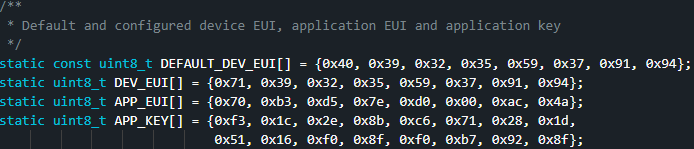
\includegraphics[width=0.85\textwidth]{images/6/Node_config.png}
        \caption{Configuration for the \texttt{OTAA} in the node}
        \label{fig:nodeconfig}
    \end{figure}
    \begin{itemize}
        \item \texttt{DEV\_EUI}: The unique identifier specified by the teachers, in this project, the first byte is $0x71$.
        \item \texttt{APP\_EUI}: The unique identifier for the end application in the network server.
        \item \texttt{APP\_KEY}: This key is used to generate the two keys for the MAC layer and the payload.
    \end{itemize}
    \item \textbf{Type of device}: the node works in class A of \acrshort{lorawan}. It will open 2 specific RX windows after a TX.
\end{itemize}

\subsection{Node definition in the network server}

In the network server, a node was defined with the next characteristics:
\begin{itemize}
    \item \textbf{Name}: \texttt{NODE\_SN\_GROUP\_A}.
    \item \textbf{Node AUTH}: \texttt{LoRaWAN OTAA Class A}.
    \item \textbf{Device EUI}: The same defined in the node configuration in \autoref{fig:nodeconfig}.
    \item \textbf{Application}: The app that shares the same \texttt{APP\_EUI} as in the \autoref{fig:nodeconfig}. In this case, \\ \texttt{RRSS2024\_AppEUI}, that has the configuration of \autoref{fig:appconfig}.
    \begin{figure}[H]
        \centering
        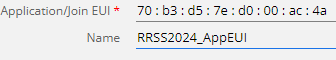
\includegraphics[width=0.6\textwidth]{images/6/AppName.png}
        \caption{App configuration in the network server}
        \label{fig:appconfig}
    \end{figure}
    \item \textbf{APP\_KEY}: The same defined in the node configuration in \autoref{fig:nodeconfig}.
    \item \textbf{LoRaWAN Network Server}: This field points to the server ``eu72.resiot.io\:7677'', configured as a \acrshort{lorawan} Europe server (\texttt{868 MHz}) for Class A+C nodes.
    \item \textbf{Advanced LoRaWAN configuration}: the most important one is that it has \acrfullr{adr}. The reception windows offset are also by default.
    \item \textbf{Node Fields}: These elements allow for dynamic updates of the dashboard. The ones defined and used are as follows:
    \begin{table}[H]
        \begin{center}
            \begin{tabular}{|p{0.20\textwidth} | p{0.20\textwidth} |c| p{0.20\textwidth}| p{0.20\textwidth}|}
                \hline
                \textbf{Field Name} & \textbf{Content Type} & \textbf{Example value} & \textbf{Predefined in the node?}\\
                \hline
                Latitude & Numeric & $40.233921051$ & Yes \\
                \hline
                Longitude & Numeric & $-3.377102145$ & Yes \\
                \hline
                Altitude & Numeric & $665$ & Yes \\
                \hline
                Altitude & Numeric & $665$ & Yes \\
                \hline
                X\_Acc & Numeric & $-0.4692$ & No \\
                \hline
                Y\_Acc & Numeric & $0.0574608$ & No \\
                \hline
                Z\_Acc & Numeric & $9.65342109375$ & No \\
                \hline
                Temperature & Numeric & $23.02$ & No \\
                \hline
                Humidity & Numeric & $54.4$ & No \\
                \hline
                Clear & Numeric & $980$ & No \\
                \hline
                Red & Numeric & $365$ & No \\
                \hline
                Green & Numeric & $383$ & No \\
                \hline
                Blue & Numeric & $346$ & No \\
                \hline
                Light & Numeric & $3.8$ & No \\
                \hline
                Moisture & Numeric & $15.8$ & No \\
                \hline
                LEDStatus & String & OFF & No \\
                \hline
            \end{tabular}
        \end{center}
        \caption{Configuration of the node fields in the ResIoT application.}
        \label{Connections3}
    \end{table}
\end{itemize}
\clearpage
\subsection{LUA Scripting}
\clearpage
\subsection{Dashboard design}
\clearpage
\clearpage
\fancyhead[R]{\textit{PROBLEMS DETECTED AND SOLUTIONS IMPLEMENTED}}
\section{PROBLEMS DETECTED AND SOLUTIONS IMPLEMENTED}
\label{problems}

\subsection{Memory limits}
As several software resources for the \acrshort{lorawan} stack were used, The amount of \acrfullr{ram} used by the system was more than the previous project without the measurement threads.

When the system was being tested, and the threads included in the project, the call to start the threads returned an \texttt{osStatus==osErrorNoMemory(0x85)}. This indicated that the 
\acrfullr{rtos}  could not allocate the stack size indicated in the constructor call for the thread.

Another factor that worsen the issue was the queue developed for the communication of the previous project. This queue needed the allocation of 
more bytes to be able to manage more structures. In reaction to this, the communication decision to use only 1 structure with a mutex was done.

Following the problems with the threads, to further understand the requirements of memory to adjust the stack size for each thread, a stack tracing tool was used\cite{Runtimememorystatistics}.

With this tool, the results in \autoref{fig:memstack} were achieved in terms on stack analysis.
\begin{figure}[H]
    \centering
    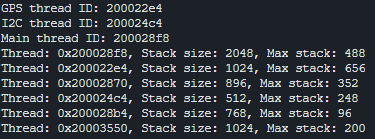
\includegraphics[width=0.7\textwidth]{images/7/Thread Traced.png}
    \caption{Threads stack usage for problem detection}
    \label{fig:memstack}
\end{figure}

As can be seen in the figure, ignoring the main thread that is not supposed to be changed, the \acrfullr{i2c} thread only uses around \texttt{248 Bytes}, while the GPS thread uses around \texttt{656 Bytes}(this is the result of the parsing of \acrfullr{nmea} data).

With this in mind, the stack were defined as follows: \texttt{512 Bytes} for the \acrshort{i2c} thread and \texttt{1024 Bytes} for the GPS thread.

\subsection{Frame size limits}

The \acrshort{lorawan} technology used in this project only allows around $1\%$ duty cycle in Europe. Because of this, it is very important for the application to use all the bits of the application message as much as possible. This allows for higher relation between transmitting windows allocation and information exchanged between the node and the network server.

In the case of the project, the frame size is \texttt{30 Bytes}, and at the start of the project, sending all the data in one single frame seemed impossible without trunking float values, which results in loss of precision.

As the user sees a lot of values that are only important as percentage, a encoding to metrics such as humidity, light and moisture was designed:
\begin{enumerate}
    \item The value is processed in the \acrfullr{mcu}, which gives a float \% value from \texttt{0.0} to \texttt{100.0} .
    \item Then, the value is multiplied by 10 and converted to an unsigned integer.
    \item Finally, as the value goes from \texttt{0} to \texttt{1000}, it can be expressed with only \texttt{10 bits}.
    \item When received in the network server, the value can be divided by 10 and we have a percentage value with at least 1 decimal, which is perfect for this use case. 
    This approach only reduces precision percentage values without trunking, while leaving full precision for the acceleration.
\end{enumerate}

This encoding gave enough room to send all the data in \texttt{29 Bytes}, and allowed the inclusion of a header byte in the frame.

\subsection{Usage of LUA 5.1}

The design solution for the frame described above created another problem in the Network Server. The Network Server script 
uses LUA 5.1, which doesn't support the most important bitwise operators\cite{luauserswikiBitwise} such as shifting.

To solve this, the next steps were taken:
\begin{enumerate}
    \item All the values that were align were send first on the frame structure.
    \item As the frame had a moment in which the byte alignment was lost, it was decided to separate acceleration values to make \texttt{3 Byte} combinations between one percentage 
    value and one acceleration axis. This meant that the bit masking and shifting operation needed to be designed once.
    \item Then, the values were obtained using the function that the ResIoT library provides and simple divisions.
\end{enumerate}

\clearpage
\fancyhead[R]{\textit{TESTING AND VALIDATION}}
\section{TESTING AND VALIDATION}
\subsection{Incremental integration and testing}

In the previous project, GIT was used to keep tracking of integration. This was also used for this project.

The workflow used was the same, each functionality, integration or implementation change was done in a separate branch and tested until it was working 
as the requirements specified it. When the functionality was working and was tested, it was merged to the main branch.

The milestones for this project were:
\begin{enumerate}
    \item Definition of the shared data for thread communications.
    \item Integration of the threads with the shared data.
    \item Refactoring of the shared data to work as a frame structure for \acrshort{lorawan}.
    \item Final testing, documentation and refactoring.
\end{enumerate}


\subsection{ResIoT testing}

Sometimes, the connection with the Network Server could not be achieved. In order to keep developing from home, the manual injection of RX events 
in the smart scripts(see \autoref{fig:manualInjection}) was used to test:
\begin{itemize}
    \item Correct decoding of not align parts of the payload.
    \item Correct format sent from the node itself.
\end{itemize}
\begin{figure}[H]
    \centering
    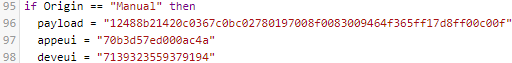
\includegraphics[width=0.9\textwidth]{images/8/manualInjection.png}
    \caption{Manual injection to test the smart script}
    \label{fig:manualInjection}
\end{figure}

\clearpage
\subsection{Code Size}
As well as the previous project, the results from the compilation in Mbed Studio is presented in the next figures. No changes to the default compilation profiles were done. 
\begin{figure}[H]
    \centering
    \begin{subfigure}[t]{0.45\textwidth}
        \centering
        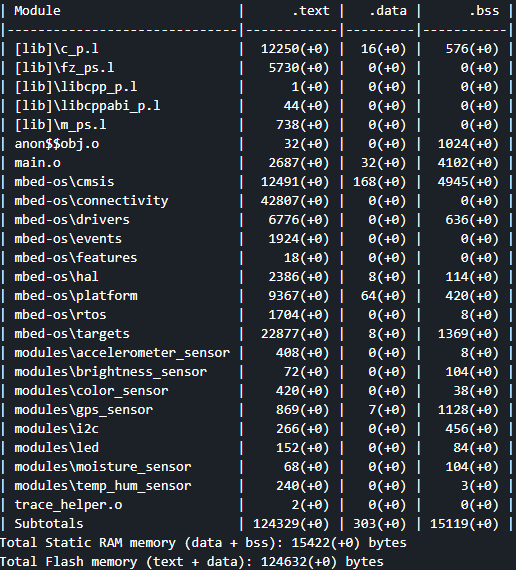
\includegraphics[width=0.882\textwidth]{images/8/debugSize.png}
        \caption{Debug compilation}
    \end{subfigure}
    \begin{subfigure}[t]{0.45\textwidth}
        \centering
        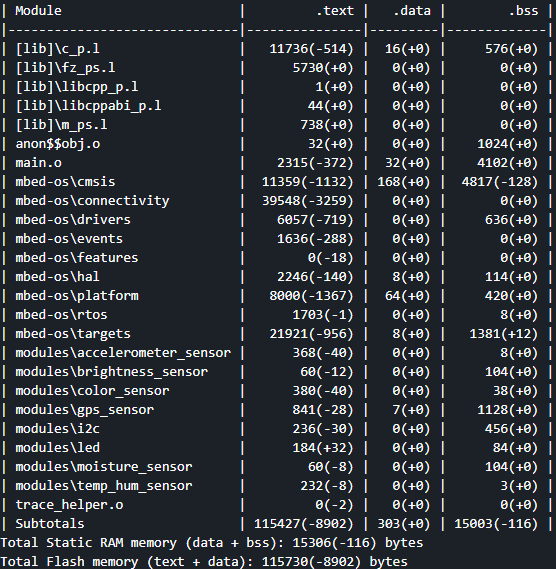
\includegraphics[width=0.95\textwidth]{images/8/developSize.png}
        \caption{Develop compilation}
    \end{subfigure}
    \begin{subfigure}[t]{0.45\textwidth}
        \centering
        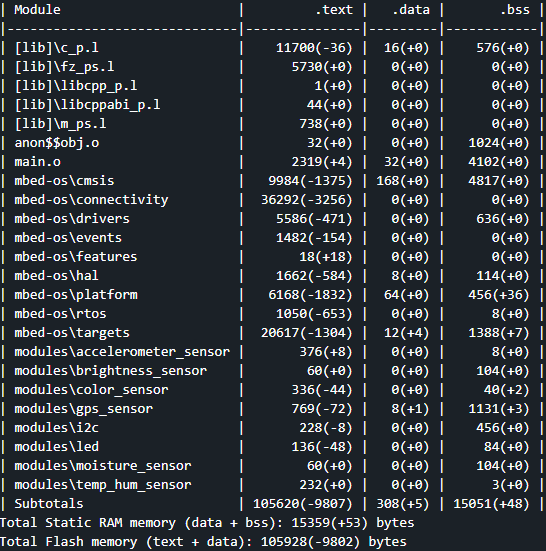
\includegraphics[width=0.95\textwidth]{images/8/releaseSize.png}
        \caption{Release compilation}
    \end{subfigure}
    \caption{Code size and module size for every compilation profile}
    \label{fig:compilation}
\end{figure}
\clearpage

\clearpage
\fancyhead[R]{\textit{DOCUMENTATION}}
\section{DOCUMENTATION}
As this project integrates different kinds of elements and software modules and all the design would be used for next subjects, it was decided that some of the efforts were going to be allocated on generating 
good documentation of the code.
\clearpage
\fancyhead[R]{\textit{RESULTS}}
\section{RESULTS}

A \acrshort{lorawan} based system was implemented from the case use study to the implementation, following all the specific requirements told by the teachers of the subject. 
To further expand the capabilities of the communications, a high amount of the efforts allocated were applied to design an advanced header and frame structure to utilize all the 
\texttt{30 Bytes} limits of \acrshort{lorawan}.

To achieve this in the time limit, a GitHub based continuous design and integration was followed. In relation to this, the project was documented with Doxygen , and deployed as a static page with GitHub actions, this information 
is available at \url{https://ryvenkappa.github.io/SensorNetworksP1/}, with the final repository of the project being at: \url{https://github.com/RyvenKappa/SensorNetworksP1}.

Finally, the project allowed the student to understand the limitations and capabilities of \acrshort{lorawan}, understanding as well the basis of the standard model design 
for \acrshort{iot} systems that integrate gateways for intercommunications.




\clearpage
\fancyhead[R]{\textit{REFERENCES}}
\printbibliography[title={REFERENCES}, heading=bibnumbered]
\clearpage
\fancyhead[R]{\textit{APPENDIX}}
\section{APPENDIX: Shared data structures}
\label{appendix}
\lstinputlisting[caption={Shared\_data.h}, label={lst:myfile}]{../modules/shared_data/shared_data.h}
\end{document}